\subsection {Ionosphere}

In the S/X geodetic system independent group delay estimates
are made for X-band and S-band, and a linear combination of these
delays,
$\tau_g=1.081 \tau_x - 0.081 \tau_s$,
is used to give a group delay measurement that is largely
free of ionospheric effects. One drawback of this system is that
both the S and X band obervations have to have a high enough 
signal-to-noise ratio so that a good detection can be made in each band.
In constrast,
the VGOS system is designed to work with very short scans, in which
the individual bands may not provide a reliable detection, and
in which all 4 bands need to be combined coherently in a fit. Since
this fit also spans a wide frequency range, it is necessary to
fit and remove the differential ionosphere from the group delay
estimate.

The phase contribution in radians due to the ionosphere, 
$\Delta \phi$, is 

\begin{equation}
        \Delta \phi = -8.448 x 10^9 \Delta TEC / f
\end{equation}
%
where f is the observing frequency in Hz, and 
$\Delta TEC \equiv TEC_a - TEC_b$ is the differential TEC
for baseline \textit{ab} in TEC units 
(1 TEC unit = $10^{16}$ elec $/ m^2$). 
\textit{NOTE! This definition of the sense of the differential
quantity as reference minus remote is (unfortunately) the opposite
of the standard used throughout the rest of fourfit.}
Since phase is only measured modulo $2\pi$, there is a non-linear
dependence of phase upon the $\Delta$TEC parameter in the
model, which restricts the manner in which a fit might
be performed.

\begin{figure}[tb]
  \centering
  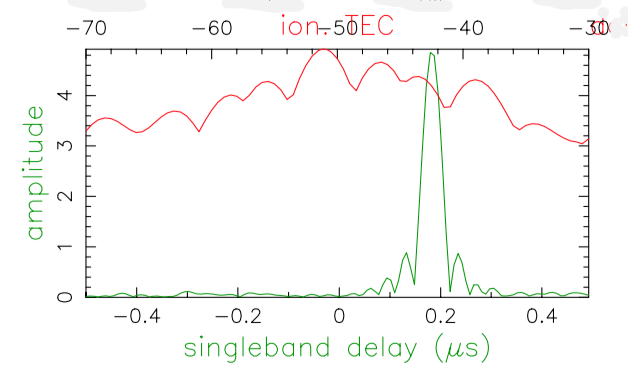
\includegraphics[width=.5\linewidth]{./ionosphere2.png}
  \caption{Ionospheric fit - correlation amplitude as a function of differential TEC
in TEC units (red curve). A complete fringe
fit at multiple points for trial values of the ionospheric
differential TEC is performed, and the code finds
the interpolated maximum.}
  \label{fig:ionosphere}
\end{figure}


The original algorithm used was that a range of coarse values 
were specified, the maximum within the range was found, then a second pass fine search
was done around the maximum. 
Recently the \textit{fourfit} code has been modified in a modest way,
in order to increase
the ionosphere search to be 3 level - (coarse, medium, fine). The
intent is to allow efficient searches over a wider range of $\Delta$TEC.

It is currently parameterized to allow a flexible coarse search, though
it is recommended that the user employs a 4 TEC unit spacing 
of the grid points over a wide range of $\Delta$TEC values. The fringe fit 
in Figure \ref{fig:ionosphere} used:
\begin{itemize}
    \item{coarse}: 11 points from (-70, -30)
    \item{medium}: 11 points with 2 unit spacing = +/- 10 units about the coarse peak
    \item{fine}: 11 points with 0.4 unit spacing = +/- 2 units about the medium peak
    \item{final}: parabolic interpolation of three fine points around the fine point peak
\end{itemize}

The medium and fine spacings are automatically generated; as before,
the user only supplies the coarse range and npts.
Though the efficiency of this algorithm could possibly
be improved, it has proven a very robust mechanism for finding the maximum value.

\subsubsection {Smoothing}

There is an option, invoked by ion\_smooth true (default: false)
in the fourfit control file. If invoked, the
code will do a 2-pass (as opposed to 3-pass) search
of TEC space, looking for the amplitude maximum. The
coarse spacing is determined by ion\_win and ion\_npts,
as before:

coarse\_step = (ion\_win[1] - ion\_win[0]) / (ion.npts - 1)

The smoothing code takes the grid points from the coarse
search and performs a convolutional smoothing, using
a half-cycle of a cosine function as the smoothing kernel.
It then finds the maximum of the smoothed, interpolated
new points. Execution of this step takes negligible time.

A final fine search is then done about the smoothed
maximum, of double width (of the non-smoothed fine search
- i.e. 24 pts) at 0.4 TEC unit spacing.

The intent of this code is to make use of the information
present over a broader range of TEC's than just the
peak. In some cases a little noise might make one
(unsmoothed) peak higher than another, but with
smoothing the peak will be brought up by the strength
of the surrounding points, at least in theory.


\subsection{Combining Linear Polarization Products}

In order to achieve reasonably good feed characterstics across the
full frequency range, the VGOS design uses linearly polarized feeds.
This adds significant complexity to the signal processing tasks, as
all 4 polarization products must be produced and then combined in an
optimal fashion to estimate group delay. A pseudo-Stokes I (Intensity)
observable can be formed, which is accurate to first order in the 
polarization leakage D-terms (Corey 2011).  The pseudo Stokes-I 
observable is formed as
\begin{equation} \label{eq:stokesI}
        I = (\overline{X_a \star X_b} + \overline{Y_a \star Y_b}) cos (\delta p) 
          + (\overline{X_a \star Y_b} - \overline{Y_a \star X_b}) sin (\delta p)
\end{equation}
where $\delta p$ is the differential
parallactic angle between sites $a$ and $b$, and $\overline{X_a \star Y_b}$ 
is (for example) the 
time-averaged correlation product of site $a$'s $X$ polarization with 
site $b$'s $Y$ polarization.
%

